%====================================================================
%====================================================================
\section*{Introduction}
%====================================================================
\frame{\frametitle{Statistical models} 

  \begin{tabular}{cc}
    \hspace{-.05\textwidth}
    \begin{tabular}{p{.7\textwidth}}
      \paragraph{Statistical modelling} typically aims at describing how
      $$
      \emphase{X =} \text{ set of descriptors = 'covariates'}
      $$ \pause
      affects the variations of 
      $$
      \emphase{Y =} \text{ set of reponse variables of interest  = 
      'response'}
      $$ \pause
      via a statistical model
      $$
      Y \sim p_\theta(\cdot \mid X) = \emphase{p_\theta}(\cdot)
      $$ \pause
      which involves
      $$
      \emphase{\theta =} \text{ unknown parameter}.
      $$
    \end{tabular}
    & 
    \hspace{-.05\textwidth}
    \begin{tabular}{c}
      \paragraph{'Graphical model':} ~ \\
      \bigskip \\
      \begin{tikzpicture}
  \node[observed] (X) at (-0.5*\edgeunit, 1*\edgeunit) {$X$};
  \node[hidden] (theta) at (0.5*\edgeunit, 1*\edgeunit) {$\theta$};
  \node[observed] (Y) at (0, 0) {$Y$};

  \draw[arrow] (X) to (Y);
  \draw[arrow] (theta) to (Y);
\end{tikzpicture}

    \end{tabular}
  \end{tabular}

  \bigskip \bigskip \pause
  \paragraph{Statistical inference:} Learn something about $\theta$ based on observed $(X, Y)$.

}

%====================================================================
\frame{\frametitle{Latent variable models} 

  \begin{tabular}{cc}
    \hspace{-.05\textwidth}
    \begin{tabular}{p{.6\textwidth}}
      \paragraph{Latent variables =} fourth actor in the play
      $$
      \emphase{Z =} \text{ set of unobserved variables}
      $$
      also affecting the variations of the response $Y$
    \end{tabular}
    & 
    \hspace{-.05\textwidth}
    \begin{tabular}{p{.6\textwidth}}
      \begin{tikzpicture}
  \node[observed] (X) at (-1*\edgeunit, 1*\edgeunit) {$X$};
  \node[hidden] (Z) at (0*\edgeunit, 1*\edgeunit) {$Z$};
  \node[hidden] (theta) at (1*\edgeunit, 1*\edgeunit) {$\theta$};
  \node[observed] (Y) at (0, 0) {$Y$};

  \draw[dashedarrow] (X) to (Z);
  \draw[arrow] (theta) to (Z);
  \draw[arrow] (X) to (Y);
  \draw[arrow] (Z) to (Y);
  \draw[arrow] (theta) to (Y);
\end{tikzpicture}

    \end{tabular}
  \end{tabular}

  \bigskip \bigskip \pause
  \paragraph{Statistical inference:} 
  Learn something about $\theta$ based on observed $(X, Y)$, that is: without observing $Z$.

  \bigskip \bigskip \pause
  \paragraph{No official distinction} between the definitions of $\theta$ and $Z$ but, often,
  \begin{itemize}
    \item $\theta =$ few interpretable parameters, 
    \item $Z \simeq$ same dimension as $Y$ itself.
  \end{itemize}

}

%====================================================================
\frame{\frametitle{Model 1: Joint species distribution model (JSDM)} 

  \paragraph{Data at hand.} $n$ sites, $p$ species, $d$ descriptors
  \medskip
  \begin{itemize}
    \setlength{\itemsep}{1.25\baselineskip}
    \item $X_i =$ environmental descriptors for site $i$
    \item $Y_i =$ species abundances in site $i$
  \end{itemize}

  \bigskip \bigskip \pause
  \paragraph{Poisson log-normal (PLN) model:} \refer{AiH89,CMR21}
  \medskip
  \begin{itemize}
    \setlength{\itemsep}{1.25\baselineskip}
    \item \pause $Z_i =$ Gaussian latent vector associated with site $i$: $Z_i \sim \Ncal_p(0, \emphase{\Sigma})$ ;
    \item \pause $Y_{ij} = $ observed abundance for species $j$ in site $i$: 
    $$
    Y_{ij} \mid Z_{ij} \sim \Fcal(x_i^\intercal \emphase{\beta_j} + Z_{ij})
    $$
    (here $\Fcal =$ Poisson)
    \item \pause Unknown parameter: ${\theta} = (\beta, \Sigma)$
  \end{itemize}

}

%====================================================================
\frame{\frametitle{Model 1: Barents' fishes}

  \begin{tabular}{cc}
    \hspace{-.04\textwidth}
    \begin{tabular}{p{.61\textwidth}}
      \paragraph{Data:} 
      \begin{itemize}
        \setlength{\itemsep}{1.25\baselineskip}
        \item $n=89$ sites, $p=30$ species, $d=4$ covariates 
        \item Abundance table: ${Y} = [Y_{ij}]$
        \item Covariate table: ${X} = [x_{ik}]$
     \end{itemize}
 
      \onslide+<2->{\bigskip \bigskip 
      \paragraph{Interpretation:} 
      \begin{itemize}
        \setlength{\itemsep}{1.25\baselineskip}
        \item \onslide+<2->{$\beta = $ regression coefficients %\\
        \ra 'abiotic' effects}
        \item \onslide+<3->{$\Sigma =$ covariance (latent layer) %\\
        \ra 'biotic' associations}
      \end{itemize}}
    \end{tabular}
    & \pause
    \hspace{-.05\textwidth}
    \begin{tabular}{p{.4\textwidth}}
      \onslide+<2->{\paragraph{Regression coefficients $\widehat{\beta}$:} 
      abiotic \\ 
      \includegraphics[width=.3\textwidth, trim=0 0 20 20, clip=]{\figeco/BarentsFish-coeffAll} \\}
      \onslide+<3->{\paragraph{Covariance matrix $\widehat{\Sigma}$:} biotic \\ 
      \includegraphics[width=.3\textwidth, trim=0 0 20 20, clip=]{\figeco/BarentsFish-corrAll}} \\
    \end{tabular}    
  \end{tabular}
}

%====================================================================
\frame{\frametitle{Model 2: Network model} 

  \paragraph{Data at hand.} $n$ species, $d$ descriptors
  \medskip
  \begin{itemize}
    \setlength{\itemsep}{1.25\baselineskip}
    \item $X_{ij} =$ similarity measure between species $i$ and $j$
    \item $Y_{ij} =$ 'interaction' intensity between species $i$ and $j$
  \end{itemize}

  \bigskip \bigskip \pause
  \paragraph{Stochastic block model (SBM):} \refer{HoL79,NoS01,MRV10}
  \medskip
  \begin{itemize}
    \setlength{\itemsep}{1.25\baselineskip}
    \item \pause $Z_i =$ latent class to which species $i$ belongs: $Z_i \sim \Mcal_K(\emphase{\pi})$ ;
    \item \pause $Y_{ij} = $ interaction intensity between species $i$ and $j$: 
    $$
    Y_{ij} \mid Z_i=k, Z_j=\ell \sim \Fcal(\emphase{\alpha_{k\ell}} + x_{ij}^\intercal \emphase{\beta})
    $$
    \item \pause Unknown parameters: ${\theta} = (\pi, \alpha ,\beta)$
  \end{itemize}

}

%====================================================================
\frame{\frametitle{Model 2: Tree interaction network} 

  \begin{tabular}{cc}
    \hspace{-.04\textwidth}
    \begin{tabular}{p{.5\textwidth}}
      \paragraph{Data:} 
      \begin{itemize}
        \setlength{\itemsep}{1.25\baselineskip}
        \item $n=51$ species, $d=1$ covariate 
        \item $Y_{ij} =$ number of fugal parasites shared by species $i$ and $j$ ($\Fcal = $ Poisson)
        \item $x_{ij} =$ taxonomic distance between species $i$ and $j$
     \end{itemize}
 
      \onslide+<2->{\bigskip \bigskip 
      \paragraph{Interpretation:} 
      \begin{itemize}
        \setlength{\itemsep}{1.25\baselineskip}
        \item \onslide+<2->{$\beta =$ regression coefficient\\
        \ra effect of the taxonomic distance}
        \item \onslide+<3->{$\pi =$ group proportions \\
        \ra distribution of the hidden groups}
        \item \onslide+<4->{$\alpha =$ group interactions \\
        \ra network structure}
      \end{itemize}}
    \end{tabular}
    & \pause
    \begin{tabular}{p{.45\textwidth}}
      \onslide+<2->{\paragraph{Estimates:}
      $\widehat{K} = 4$, $\widehat{\beta} = -.317$. \\
      }
      \onslide+<3->{\paragraph{Group proportions:} \\ 
        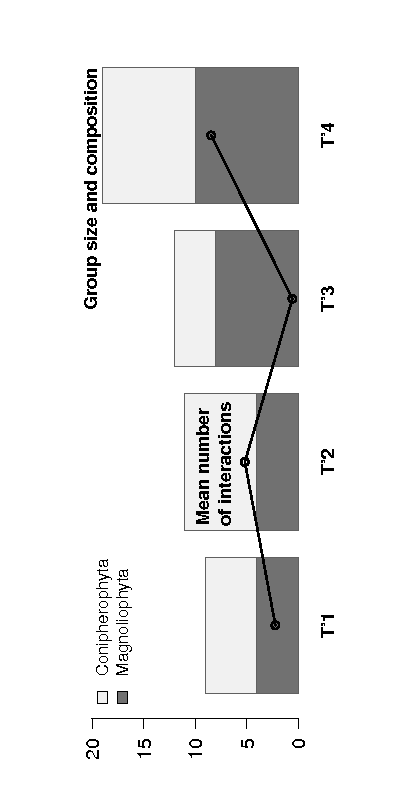
\includegraphics[height=.2\textwidth, width=.3\textwidth, trim=150 200 150 200, clip=]{\fignet/MRV10_AoAS_Q4_group} \\} 
      \onslide+<4->{\paragraph{Group interactions:} \\ 
        \includegraphics[height=.3\textwidth, width=.3\textwidth]{\fignet/Tree-adjMat-SBMtaxo}} 
    \end{tabular}    
  \end{tabular}
  
}

%====================================================================
\frame{\frametitle{Some differences} 

  \paragraph{Nature of the latent variables:}
  \begin{itemize}
    \setlength{\itemsep}{1.25\baselineskip}
    \item \emphase{Species abundance =} continuous, multivariate (Gaussian)
    \item \emphase{Network =} univariate, discrete (multinomial)
  \end{itemize}
  
  \bigskip \bigskip \pause
  \paragraph{Modeling function of the latent variables:}
  \begin{itemize}
    \setlength{\itemsep}{1.25\baselineskip}
    \item \emphase{Species abundance =} instrumental: comfortable multivariate Gaussian setting \\
    \ra no precise ecological interpretation of the $Z_i$ \\
    \ra focus on the inference of the parameter $\theta = (\beta, \Sigma)$
    \item \emphase{Network =} 'mechanistic': hopefully, species groups have an ecological meaning \\
    \ra easier interpretation of the $Z_i$ \\
    \ra focus on unsupervised classification
  \end{itemize}
  
  \bigskip \bigskip \pause
  \paragraph{Many other typical uses of latent variable:} modelling time, space or time-space dependencies

}

%====================================================================
\frame{\frametitle{Latent variable models in ecology \refer{PeG22b}} 

  $$
  \begin{tabular}{cc}
%     \includegraphics[height=.6\textheight]{\fig/PeG22-Fr-BookCover} & 
    \includegraphics[height=.6\textheight]{\fig/PeG22-En-BookCover}
  \end{tabular}
  $$
  (French version: \refer{PeG22a}).

}

